\section{Design Options}

\mnote{Space of design options}
The development of a language for realizing the \commonalities approach offers several degrees of freedom.
They range from conceptual degrees of freedom, e.g., regarding the operationalization alternatives discussed in \autoref{chap:improvement:commonalities:operationalization}, over notation types, such as textual or graphical representations, to the specific syntax to use or even reuse from existing languages.
We, in particular, consider the conceptual degrees of freedom and give an overview of how an according textual syntax can look like.

\mnote{Operationalization options}
The conceptual degrees of freedom include options for operationalizing a specification in terms of using the \conceptmetamodels as additional metamodels with the manifestation relations constituting ordinary transformations, or in terms of generating direct transformations between the \concretemetamodels from the \commonalities specification, as both discussed in \autoref{chap:improvement:commonalities:operationalization}.
This option selection is transparent to the developer of a transformation network, as it only affects its operationalization.

\mnote{Specification options}
In addition, we can distinguish \emph{internal} and \emph{external} specifications, depending on whether the specification is decomposed by the \commonalities or by the defined manifestation relations.
This decision affects the developer of a transformation network, as he or she is directly concerned with the way in which \commonalities are specified.
We discuss these two options in the following in more detail.
Furthermore, we derive an overview of the resulting process for specifying and executing artifacts in such a language.


\subsection{Internal and External Specification}
\label{chap:language:design:internal_external}

\begin{figure}
    \centering
    \newcommand{\distance}{4em}
\newcommand{\vdistance}{2.5em}
\newcommand{\scenariodistance}{4*\distance+0.6*\difftoafiveimage}
\newcommand{\overlapdistance}{0.3em}

\begin{tikzpicture}[
    manifests relation label/.style={manifests relation, above, sloped}
]

% EXTERNAL CONCEPT DEFINITION

\node[schematic conceptmetamodel] (cmm_concept1) {};
\node[schematic conceptmetamodel, right=\overlapdistance of cmm_concept1.center, anchor=center] (cmm_concept2) {};
\node[schematic conceptmetamodel, right=\overlapdistance of cmm_concept2.center, anchor=center] (cmm_concept3) {};

\node[schematic conceptmetamodel, right=\distance of cmm_concept1.center, anchor=center] (cmm_rel1_concept1) {};
\node[schematic conceptmetamodel, right=\overlapdistance of cmm_rel1_concept1.center, anchor=center] (cmm_rel1_concept2) {};
\node[schematic conceptmetamodel, right=\overlapdistance of cmm_rel1_concept2.center, anchor=center] (cmm_rel1_concept3) {};

\node[schematic metamodel, below left=\vdistance and 0.2*\distance of cmm_rel1_concept1.center, anchor=center] (cmm_rel1_concrete1) {};
\node[schematic metamodel, right=\overlapdistance of cmm_rel1_concrete1.center, anchor=center] (cmm_rel1_concrete2) {};
\node[schematic metamodel, right=\overlapdistance of cmm_rel1_concrete2.center, anchor=center] (cmm_rel1_concrete3) {};

\node[schematic conceptmetamodel, right=\distance of cmm_rel1_concept1.center, anchor=center] (cmm_rel2_concept1) {};
\node[schematic conceptmetamodel, right=\overlapdistance of cmm_rel2_concept1.center, anchor=center] (cmm_rel2_concept2) {};
\node[schematic conceptmetamodel, right=\overlapdistance of cmm_rel2_concept2.center, anchor=center] (cmm_rel2_concept3) {};

\node[schematic metamodel, below right=\vdistance and 0.2*\distance of cmm_rel2_concept1.center, anchor=center] (cmm_rel2_concrete1) {};
\node[schematic metamodel, right=\overlapdistance of cmm_rel2_concrete1.center, anchor=center] (cmm_rel2_concrete2) {};
\node[schematic metamodel, right=\overlapdistance of cmm_rel2_concrete2.center, anchor=center] (cmm_rel2_concrete3) {};

\draw[manifests relation] (cmm_rel1_concept1) -- (cmm_rel1_concrete1);
\draw[manifests relation] (cmm_rel1_concept2) -- (cmm_rel1_concrete2);
\draw[manifests relation] (cmm_rel1_concept3) -- (cmm_rel1_concrete3);

\draw[manifests relation] (cmm_rel2_concept1) -- (cmm_rel2_concrete1);
\draw[manifests relation] (cmm_rel2_concept2) -- (cmm_rel2_concrete2);
\draw[manifests relation] (cmm_rel2_concept3) -- (cmm_rel2_concrete3);

\node[below right=0.5*\vdistance and 0.5*\distance of cmm_concept2.center, anchor=center, font=\bfseries] {+};
\node[below right=0.5*\vdistance and 0.5*\distance of cmm_rel1_concept2.center, anchor=center, font=\bfseries] {+};


% INTERNAL CONCEPT DEFINITION

\node[schematic conceptmetamodel, right=\scenariodistance of cmm_concept1.center, anchor=center] (int_concept1) {};
\node[schematic metamodel, below left=\vdistance and 0.2*\distance of int_concept1.center, anchor=center] (int_concept1_concrete1) {};
\node[schematic metamodel, below right=\vdistance and 0.2*\distance of int_concept1.center, anchor=center] (int_concept1_concrete2) {};
\draw[manifests relation] (int_concept1) -- (int_concept1_concrete1);
\draw[manifests relation] (int_concept1) -- (int_concept1_concrete2);

\node[schematic conceptmetamodel, right=\distance of int_concept1.center, anchor=center] (int_concept2) {};
\node[schematic metamodel, below left=\vdistance and 0.2*\distance of int_concept2.center, anchor=center] (int_concept2_concrete1) {};
\node[schematic metamodel, below right=\vdistance and 0.2*\distance of int_concept2.center, anchor=center] (int_concept2_concrete2) {};
\draw[manifests relation] (int_concept2) -- (int_concept2_concrete1);
\draw[manifests relation] (int_concept2) -- (int_concept2_concrete2);

\node[schematic conceptmetamodel, right=\distance of int_concept2.center, anchor=center] (int_concept3) {};
\node[schematic metamodel, below left=\vdistance and 0.2*\distance of int_concept3.center, anchor=center] (int_concept3_concrete1) {};
\node[schematic metamodel, below right=\vdistance and 0.2*\distance of int_concept3.center, anchor=center] (int_concept3_concrete2) {};
\draw[manifests relation] (int_concept3) -- (int_concept3_concrete1);
\draw[manifests relation] (int_concept3) -- (int_concept3_concrete2);

\node[below right=0.5*\vdistance and 0.5*\distance of int_concept1.center, anchor=center, font=\bfseries] {+};
\node[below right=0.5*\vdistance and 0.5*\distance of int_concept2.center, anchor=center, font=\bfseries] {+};

\node[above=0.5em of cmm_rel1_concept2.north, anchor=south, font=\small\bfseries] (ext_label) {External Concept Definition};
\node[above=0.5em of int_concept2.north, anchor=south, font=\small\bfseries] (int_label) {Internal Concept Definition};

\node[below=1.7*\vdistance of cmm_rel1_concept2.center, anchor=center, font=\footnotesize\itshape] (ext_dim_label) {Decomposition Dimension: Relations};
\node[below=1.7*\vdistance of int_concept2.center, anchor=center, font=\footnotesize\itshape] (int_dim_label) {Decomposition Dimension: Commonalities};

\draw[gray, thin] ($(ext_label.north)!0.5!(int_label.north)$) -- ($(ext_dim_label.south)!0.5!(int_dim_label.south)$);


\end{tikzpicture}
    %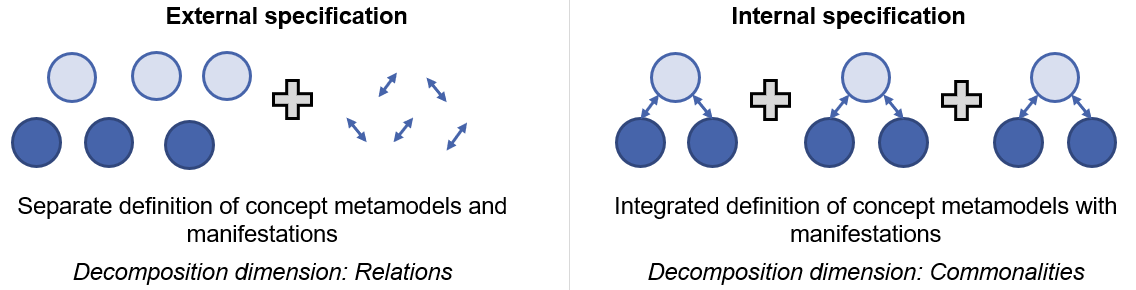
\includegraphics[width=\textwidth]{figures/quality/language/design_options.png}
    \caption[Design options for \commonalities specification]{Exemplification of alternatives to specify \commonalities by means of a separate, external specification of complete \conceptmetamodels and manifestation relations or an integrated, internal definition of \commonalities with their manifestation relations. Circles denote \commonalities and manifestations, arrows denote manifestation relations.}
    \label{fig:language:design_options}
\end{figure}

\mnote{Decomposition dimensions}
We can distinguished two ways in which \conceptmetamodels and manifestation relations can be specified according to the \commonalities approach.
They depend on the dimension along which the specification is decomposed.
More precisely, the specification can either be decomposed along the \commonalities, such that each \commonality together with all its manifestations is defined at one place, or it can be decomposed along the manifestation relations, such that all manifestation relations between a \conceptmetamodel and its manifestation are defined at one place.
We refer to these specifications as \emph{internal} and \emph{external} specifications, which we have already proposed in previous work~\owncite{klare2019models} and which we illustrate in \autoref{fig:language:design_options}.
\begin{properdescription}
    \item[External Concept Definition:] \Conceptmetamodels are defined as ordinary metamodels and each manifestation relation is defined as an individual transformation, i.e., manifestation relations are defined externally to the \conceptmetamodels and their \commonalities.
    \item[Internal Concept Definition:] Each \commonality of each \conceptmetamodel is defined together with its relations to manifestations, thus manifestation relations are defined internally with the \commonalities they belong to.
\end{properdescription}
%We call the former way an \emph{internal} specification and the latter an \emph{external} specification, related to whether relations are defined internally with the \commonalities they belong to or as an external artifact.
%We have proposed this distinction in previous work~\owncite{klare2019models} and depict it in \autoref{fig:language:design_options}.

\mnote{External specification}
Without developing an additional language, the \commonalities approach can be realized by developing \conceptmetamodels as if they are ordinary metamodels with appropriate modeling tools.
The manifestation relations can then be defined with any existing transformation language that is able to generate incremental transformations. %, i.e., consistency preservation rules.
This conforms to an \emph{external} specification, in which \conceptmetamodels and manifestation relations are defined separately.
It decomposes the specification along the relations, such that there are as many separate artifacts as there are \conceptmetamodels and relations to be defined. %, as depicted in the left of \autoref{fig:language:design_options}.
For example, for Java and \gls{UML} an object-oriented design \conceptmetamodel as well as two manifestation relations to each of the \concretemetamodels would be defined separately.

\mnote{Internal specification}
Developing a specific language allows to integrate the definition of \commonalities with their manifestation relations.
The relations to manifestations of a \commonality are then defined at one place with the declaration of the \commonality, improving locality of this related information.
This conforms to an \emph{internal} specification.
It decomposes the specification along the \commonalities, thus as many separate specifications exist as \commonalities are defined. %, as depicted in the right of \autoref{fig:language:design_options}.
For example, for Java and \gls{UML} a class \commonality together with its manifestation as classes in both Java and \gls{UML} with the according relations of attribute values and references would be defined at one place.

\mnote{Tyranny of dominant decomposition}
Selecting one of these types of specification suffers from the \enquote{tyranny of the dominant decomposition}~\cite{tarr1999Tyranny-ICSE}.
Thus, decomposition is only possible along one dimension of concerns, i.e., either the structural specification of \commonalities or the relational specification of manifestation relations, such that either one suffers from lacking separation of concerns in the other dimension.
Thus, while one approach improves locality when adding \commonalities, the other improves locality when adding manifestation relations.

\mnote{External specification benefits}
External specifications benefit from the separation of each manifestation relation into its own specification.
This reduces dependencies between the manifestations and especially allows each developer who is responsible for a specific \concretemetamodel to define the relation to each related \conceptmetamodel as a whole instead of distributing this specification among all \commonalities specifications describing a concept represented in the \concretemetamodel.
In consequence, adding a new \concretemetamodel only requires the addition and potentially adaptation of manifestation relations to \conceptmetamodels.
External specifications support this scenario well because of high locality of all information regarding a manifestation relation, and because manifestation relations represent the largest part of the addition.
Additionally, they can be realized without developing a new language.

\mnote{Internal specification benefits}
Internal specifications require a dedicated language enabling the integrated specification of \commonalities and their manifestations.
This improves locality regarding the information about each \commonality, as each \commonality is represented along with all its manifestations.
In consequence, when initially developing \commonalities for a set of \concretemetamodels, it is easier to add each single \commonality, because all information about the \commonality and its relations to the manifestations can be defined at one place.
This can make it easier to understand the overall relation of that common concept among all \concretemetamodels.
In addition, it makes it less likely for a developer to miss the definition of one or more manifestations of a \commonality, as they are obviously missing in the specification of the \commonality, whereas in an external specification it is missing somewhere in the complete manifestation relation between the \conceptmetamodel and its manifestation.
Finally, the approach promises to be more concise, because the manifestation relations are defined within the \commonality they belong to instead of referencing the \commonality within a transformation again.

\mnote{Proposal of internal specification language}
To benefit from locality regarding each \commonality and a more concise specification, we have decided to design a language that supports internal specifications.
Depending on the usage context and usual change scenarios, an external specification may, however, be more appropriate.
Then, modeling \concretemetamodels with an existing modeling framework and the manifestation relations with existing transformation languages is sufficient.


\subsection{Artifacts and Process}
\label{chap:language:design:artifacts_process}

\mnote{Selected design options}
Regarding the design options in \autoref{chap:improvement:commonalities:operationalization} and \autoref{chap:language:design:internal_external}, we have made the following, already argued decisions.
First, we chose to operationalize a specification by treating \conceptmetamodels as ordinary metamodels, such that instances of them are created and kept consistent.
This option does especially not restrict expressiveness of the relations, and the generation of additional models can be hidden from the user by appropriate tooling.
Second, we chose to provide a language that supports an internal specification of concepts to improve locality of the information regarding each \commonality.
We expect this specification to be more concise and to better support the initial specification process for \commonalities.

\begin{figure}
    \centering
    \newcommand{\developstext}{«develops»}
\newcommand{\modifiestext}{«modifies»}
\newcommand{\vdistance}{5em}
\newcommand{\hdistance}{(\vdistance+0.19*\difftoafiveimage)}

\newcommand{\tikzsystemborder}[2]{
    \node[draw, runtime artifact, ellipse, minimum width=0.5*\vdistance, minimum height=0.5*\vdistance, anchor=center, #1] (#2) {};
}

\newcommand{\tikzconcretemetamodels}[1]{
    \node[draw, runtime artifact, ellipse, minimum width=0.05*\vdistance, minimum height=0.05*\vdistance, above left=0.02*\vdistance and 0.08*\vdistance of 
    #1.center, inner sep=0em] (#1model1) {};
    \node[draw, runtime artifact, ellipse, minimum width=0.05*\vdistance, minimum height=0.05*\vdistance, above right=0.08*\vdistance and 0.04*\vdistance of #1.center, inner sep=0em] (#1model2) {};
    \node[draw, runtime artifact, ellipse, minimum width=0.05*\vdistance, minimum height=0.05*\vdistance, below right=0.08*\vdistance and 0.04*\vdistance of #1.center, inner sep=0em] (#1model3) {};
}

\newcommand{\tikzconceptmetamodels}[1]{
    %\node[draw, orchestration artifact, ellipse, minimum width=0.05*\vdistance, minimum height=0.05*\vdistance, above left=0.08*\vdistance and 0.05*\vdistance of #1.center, inner sep=0em] (#1model1) {};
    \node[draw, orchestration artifact, ellipse, minimum width=0.05*\vdistance, minimum height=0.05*\vdistance, right=0.08*\vdistance of #1.center, inner sep=0em] (#1model2) {};
    \node[draw, orchestration artifact, ellipse, minimum width=0.05*\vdistance, minimum height=0.05*\vdistance, below left=0.06*\vdistance and 0.05*\vdistance of #1.center, inner sep=0em] (#1model3) {};
}

\newcommand{\tikzconceptandconcretemetamodels}[1]{
    \tikzconcretemetamodels{#1}
    \tikzconceptmetamodels{#1}
}

\newcommand{\tikzsystemwithconcepts}[2]{
    \tikzsystemborder{#1}{#2}
    \tikzconceptandconcretemetamodels{#2}
}

\newcommand{\machine}[2]{
    \draw[#2] ([xshift=-0.5em, yshift=-0.5em]#1) -- ++(0,1em) -- ++(-0.5em, 0.5em) -- ++(2em, 0) -- ++(-0.5em, -0.5em) -- ++(0,-1em) -- ++(-1em,0);
}


\begin{tikzpicture}[
    every node/.append style={font=\footnotesize},
    developer artifact/.style={consistencypreservationcolor},
    runtime artifact/.style={},
    orchestration artifact/.style={executioncolor},
    artifact role name/.style={font=\footnotesize\bfseries}
]

% Commonalities
\node[draw, developer artifact, fill=white, inner sep=0.15em, align=left] (trans1) {
    \begin{lstlisting}[language=commonalities, frame=none, numbers=none, backgroundcolor=\color{white}, linewidth=14pt, basicstyle=\fontsize{2}{2.4}\selectfont\ttfamily]
commonality R {
  with A
  with B
    
  has att {
    = A.att
    -> B.att
  }
}
    \end{lstlisting}
};
\node[draw, below right=0.2em of trans1.north, anchor=north, developer artifact, fill=white, inner sep=0.15em, align=left] (trans2) {
    \begin{lstlisting}[language=commonalities, frame=none, numbers=none, backgroundcolor=\color{white}, linewidth=14pt, basicstyle=\fontsize{2}{2.4}\selectfont\ttfamily]
commonality R {
  with A
  with B
    
  has att {
    = A.att
    -> B.att
  }
}
    \end{lstlisting}
};
\node[draw, below right=0.2em of trans2.north, anchor=north, developer artifact, fill=white, inner sep=0.15em, align=left] (trans3) {
    \begin{lstlisting}[language=commonalities, frame=none, numbers=none, backgroundcolor=\color{white}, linewidth=14pt, basicstyle=\fontsize{2}{2.4}\selectfont\ttfamily]
commonality R {
  with A
  with B
    
  has att {
    = A.att
    -> B.att
  }
}
    \end{lstlisting}
};

% Expert
\umlhuman{expert1}{}{above left=0.2em and 1.2*\hdistance of trans2.center, anchor=center}{}{0.3}
\draw[-latex] ([yshift=-0.2em]expert1.east) -- node[above, stereotype] {\developstext} ([xshift=-0.2em]trans2.west);

% Concrete metamodels
\coordinate (concrete_metamodels) at ([yshift=\vdistance]trans2);
\tikzconcretemetamodels{concrete_metamodels}

\draw[-latex, densely dashed] ([yshift=0.2em]trans2.north) -- node[left, stereotype, align=center] {«refers\\ to»} ([yshift=-1em]concrete_metamodels);

% Compiler
\coordinate (compiler) at ([xshift=0.8*\hdistance]trans2.center);
\machine{compiler}{}

\draw[-latex] ([xshift=0.5em]trans2.east) -- ([xshift=-1em]compiler);
\draw[-latex] ([yshift=-0.5em,xshift=0.8em]concrete_metamodels) -- ([yshift=1.2em,xshift=-0.7em]compiler);

% Generated BX
\node[draw, right=1.6*\hdistance of trans1.center, anchor=center, orchestration artifact, fill=white, inner sep=0.15em, align=left] (bx1) {
    \begin{lstlisting}[language=reactions, frame=none, numbers=none, backgroundcolor=\color{white}, linewidth=14pt, basicstyle=\fontsize{2}{2.4}\selectfont\ttfamily]
reaction RAB {
  after ...
  call S
}

routine S {
  match ... 
  action ...
}
    \end{lstlisting}
};
\node[draw, below right=0.2em of bx1.north, anchor=north, orchestration artifact, fill=white, inner sep=0.15em, align=left] (bx2) {
    \begin{lstlisting}[language=reactions, frame=none, numbers=none, backgroundcolor=\color{white}, linewidth=14pt, basicstyle=\fontsize{2}{2.4}\selectfont\ttfamily]
reaction RAB {
  after ...
  call S
}

routine S {
  match ... 
  action ...
}
    \end{lstlisting}
};
\node[draw, below right=0.2em of bx2.north, anchor=north, orchestration artifact, fill=white, inner sep=0.15em, align=left] (bx3) {
    \begin{lstlisting}[language=reactions, frame=none, numbers=none, backgroundcolor=\color{white}, linewidth=14pt, basicstyle=\fontsize{2}{2.4}\selectfont\ttfamily]
reaction RAB {
  after ...
  call S
}

routine S {
  match ...
  action ...
}
    \end{lstlisting}
};

% All metamodels
\coordinate (all_metamodels) at ([yshift=\vdistance]bx2);
\tikzconceptandconcretemetamodels{all_metamodels}

\draw[-latex, orchestration artifact] ([yshift=1.2em,xshift=0.7em]compiler) -- ([yshift=-0.5em,xshift=-0.8em]all_metamodels);
\draw[-latex] ([xshift=1em]compiler) -- ([xshift=-0.5em]bx2.west);

\coordinate (upperend_all_metamodels) at ([xshift=0.2*\hdistance,yshift=0.2*\vdistance]all_metamodels);
\draw [orchestration artifact, decorate,decoration={brace,amplitude=10pt},xshift=0pt,yshift=4pt]
([xshift=0.5em]bx3.south east|-upperend_all_metamodels) -- ([xshift=0.5em]bx3.south east);

% Machine
\coordinate (machine) at ([yshift=0.2*\vdistance,xshift=2.1*\hdistance]bx2);
\machine{machine}{orchestration artifact}

\coordinate (output_middle) at ($(bx3.south east)!0.5!(upperend_all_metamodels)$);
\draw[orchestration artifact, densely dashed, -latex] ([xshift=10pt+0.5em]output_middle) -- node[below=0.2em, stereotype, align=center] {Transformation\\ Network} ([yshift=0.3em, xshift=-0.9em]machine.west);

% Input
\tikzsystemwithconcepts{above left=0.6*\vdistance and 0.48*\hdistance of machine}{original_system}
\node[runtime artifact, above=1.2em of original_system.north, anchor=south, align=center, artifact role name] {System\\ (Concrete +\\ {\color{darkorange} Concept}\\ Models)};
\node[runtime artifact, below right=0em and \hdistance of original_system.center, anchor=north] (original_changes) {$\sequenced{\change{1}, \change{2}, \change{3}, \dots}$};
\node[runtime artifact, above=-0.3em of original_changes.north east, anchor=south east, artifact role name] {Changes};

\umlhuman{developer}{}{above right=0.5*\vdistance and 0.2*\hdistance of original_changes.north, anchor=south}{}{0.3}

\draw[-latex] (developer) -- node[stereotype, sloped, above] (modifies_label) {\modifiestext} (original_system);
\draw[dashed, -latex] (modifies_label.south) -- ([xshift=-1.2em]original_changes.north);

\draw [runtime artifact, decorate,decoration={brace,amplitude=10pt},xshift=0pt,yshift=-4pt]
(original_changes.south east) -- (original_system.west|-original_system.south);

\draw[gray, densely dashed, -latex] ([xshift=-0.2em]original_system.west) -- node[above, sloped, stereotype, align=center, pos=0.35] {«instan-\\ tiates»} ([xshift=0.2em+0.25*\vdistance]all_metamodels);

% Output
\tikzsystemwithconcepts{below=0.5*\vdistance of machine}{final_system}
\node[runtime artifact, left=0em of final_system.west, anchor=east, align=center, artifact role name] {Consistent\\ System\\ (Models)};
\draw[runtime artifact, -latex] ([yshift=-0.8em]machine.south) -- ([yshift=0.2em]final_system.north); 

% Labels
\node[above=1.5em of concrete_metamodels.north, anchor=south, artifact role name, align=center, inner sep=0em] (concrete_metamodels_label) {Concrete\\ Metamodels};
\node[above=1.5em of all_metamodels.north, anchor=south, artifact role name, align=center, inner sep=0em] (concrete_metamodels_label) {Concrete +\\ {\color{darkorange} Concept}\\ Metamodels};
\node[above right=0.3em and 0.1*\hdistance of expert1.north, anchor=south, artifact role name, align=center, inner sep=0em] (expert_text) {Domain\\ Expert};
\node[developer artifact, below=0.8em of trans2.south, anchor=north, artifact role name, align=center] (comm_spec_label) {Commonalities\\ Specifications};
\node[anchor=north, below=0.8em of compiler, anchor=north, artifact role name, align=center] %at (compiler|-comm_spec_label.north) 
{Compiler};
\node[orchestration artifact, below=0.8em of bx2.south, anchor=north, artifact role name, align=center] (bx_spec_label) {Bidirectional\\ Transformations};
\node[above=0.2em of developer.north, anchor=south, artifact role name, inner sep=0em, align=center] {System\\ Developer};


\end{tikzpicture}

    %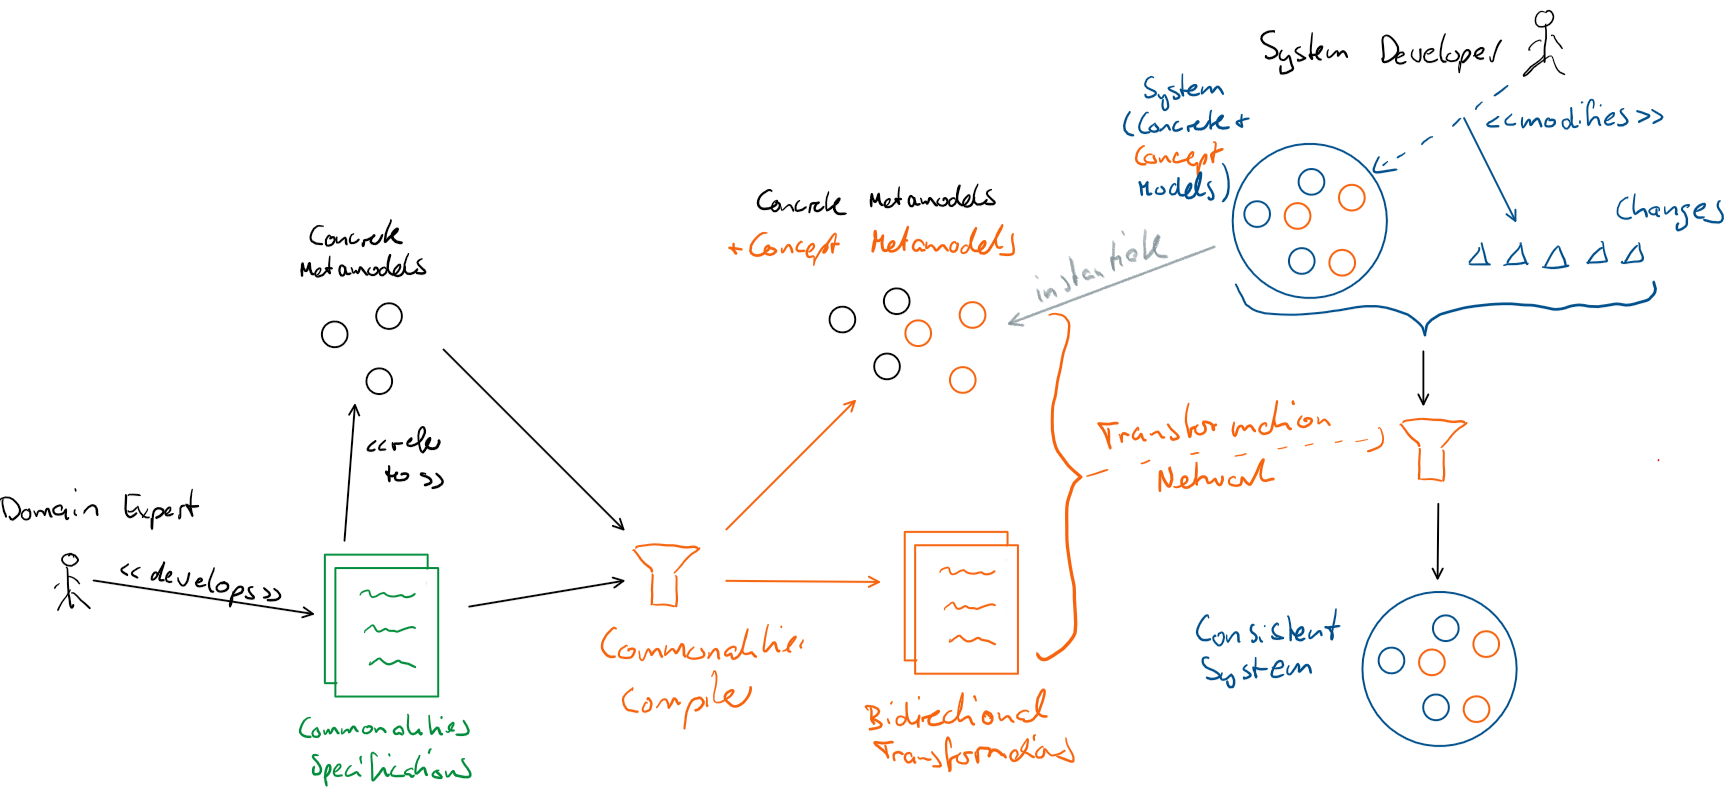
\includegraphics[width=\textwidth]{figures/quality/language/overall_process.png}
    \caption[Process and artifacts using a language for \commonalities]{The process for developing, compiling and executing specifications in a language for \commonalities. From \concretemetamodels and \commonalities specifications, additional \conceptmetamodels and transformations are generated, which are executed at runtime for preserving consistency of models.
    \Commonalities specifications by domain experts are marked orange, the generated artifacts (\conceptmetamodels and transformations forming a network) are marked green. Concrete systems and changes depict runtime artifacts.}
    \label{fig:language:process}
\end{figure}

\mnote{Specification and compilation}
The process of specifying, compiling and executing artifacts in such a language is depicted in \autoref{fig:language:process}.
It is a specialization of the general process already depicted in \autoref{fig:introduction:process_overview}.
A domain expert or transformation developer defines \commonalities specifications using the language, which refers to \concretemetamodels that are to be kept consistent by the transformations derived from that specification.
The compiler of the language takes the \concretemetamodels together with the specifications to generate a set of \conceptmetamodels in addition to the existing \concretemetamodels, as well as a set of bidirectional transformations, which implement consistency preservation for the manifestation relations between the \conceptmetamodels and \concretemetamodels.
These artifacts together form a transformation network, as introduced in \autoref{def:transformationnetwork}.

\mnote{Execution}
A system developer specifies a system by models that instantiate the \concretemetamodels of the \commonalities specification.
The complete system description consists of instances of these \concretemetamodels, but also, in the best case hidden from developer, of instances of the \conceptmetamodels for means of consistency preservation.
Whenever the system developer produces changes to the instances of the \concretemetamodels, the transformation network can be applied to the changes together with the models.
It then returns a new set of instances of the \concretemetamodel and \conceptmetamodels that are consistent again, according to the proposed correctness notion of transformation networks in \autoref{def:transformationnetworkcorrectness}.


%\begin{copiedFrom}{VoSE}

% In this paper, we present the \emph{\commonalities approach}. %, which is based on the Bachelor's thesis of \textowncite{gleitze2017a}.
% % Vorschlag:
% It defines \commonalities between metamodels explicitly and thereby allows to state clearly which common concepts they share.
% %, instead of encoding this information implicitly in a transformation.
% %The approach aims to explicitly define commonalities of metamodels for describing their consistency relations rather than implicitly encoding them in a transformation.
% From such a specification, transformations are derived that keep instances of those metamodels consistent.
% We discuss options how to derive such transformations, strategies to hierarchically compose \commonalities, as well as benefits and limitations of the approach.
% Additionally, we discuss design options for a language that supports the specification of \commonalities and present the \emph{\commonalities language}, which we have developed as a proof-of-concept.
% It is based on the Bachelor's thesis of \textowncite{gleitze2017a}.

% Having introduced the concepts of the \commonalities approach, we now present the \commonalities language, as proposed by \textowncite{gleitze2017a}.
% The language is a prototypical realization of the approach.
% We discuss design options for such a language and outline its syntax and its usage.
% This forms our contribution~\autoref{contrib:quality:language}.
% For a detailed discussion of the language capabilities, we refer to~\owncite{gleitze2017a}.
% In this paper, we focus on the presentation of fundamental concepts  and therefore only outline the language to give an impression of what our proof-of-concept evaluation is based on.


% \section*{Design Options}

% The development of a language for realizing the \commonalities approach provides at least two areas of design options.
% First, there are different possibilities to operationalize the approach, which covers decisions that are not visible to the user of the language.
% Second, different options regarding how to specify \conceptmetamodels and their relations to their manifestations exist, which are decisions that are visible to the user of the language.

% We already discussed in \autoref{chap:improvement:commonalities:operationalization} that there are two different options for operationalizing a specification of \commonalities: one that uses instances of the concept metamodels and defined transformations at runtime, and one that generates direct transformations between the \concretemetamodels from the specification.
% Since the way a specification is operationalized does not affect the user of the approach, it is up to the language and its designer to choose one of the options.
% We chose to build a language following the former approach, because it does not limit the possible relations that can be expressed.
% %We chose to build a language following the former approach, because it produces less initial effort to achieve a proof-of-concept that can be used to validate whether the approach is promising at all.

% Regarding the specification of \conceptmetamodels and the transformations, there are two options:
% \begin{description}[leftmargin=\parindent]
%     \item[External concept definition:] \Conceptmetamodels are defined as ordinary metamodels and the relations to their manifestation are defined in an individual transformation specification %, or even specifications in ordinary transformation languages, 
%     for each manifestation. %$\Rightarrow$ Benefit: Each Mapping independently specifiable
%     \item[Internal concept definition:] A specialized language allows to define the \conceptmetamodel and the \commonalities it consists of together with relations of all \commonalities to their manifestations. %$\Rightarrow$ Benefit: No elements accidentally missed \todoAll{Really or is there another benefit?}
% \end{description}

% A benefit of the first option is that the relation to each manifestation can be specified independently, which reduces dependencies between the different manifestations of one \conceptmetamodel.
% Additionally, it could be realized without developing a new language. The \conceptmetamodels can be described just like any other ordinary metamodel and one can use any existing transformation language, such as QVT, for the transformation definitions.
% The second option, in contrast, requires a dedicated language that enables an integrated specification of the \conceptmetamodel and its relations to manifestations.
% We chose to build a language following the second option because we expect its benefits to outweigh the mentioned disadvantages.
% First, it improves locality: all information about one \commonality is represented in one place.
% %instead of separating the \commonality definition from the transformation specifications.
% Because of that, we expect that it is easier for developers to understand the combined transformation logic concerning one \commonality.
% Additionally, the \conceptmetamodel can be easily extended with this solution whenever adding a manifestation requires defining a new \commonality.
% Finally, we expect that, compared to other options, grouping transformations by their \commonality reduces the possibility for developers to forget defining one or more relevant manifestations for a \commonality.
% %Finally, it is easier to ensure that for all \commonalities a relation to the manifestation is defined than in the first option, where \commonality specification and relation specification are separated.
% %Nevertheless, an obvious drawback of the second option in contrast to the first is that the mappings to the concrete metamodels cannot be specified independently but are tied to the Commonality definition.
% %Additionally, we expect that it makes it easier to understand the semantics of a \commonality and how it relates to its manifestations.}
% %and ensure that no elements are specified in the \conceptmetamodel that do have no manifestation in all relevant \concretemetamodels.

%\end{copiedFrom} % Models VoSE